\documentclass[a4paper,12pt]{article} % тип документа

% Поля страниц
\usepackage[left=2.5cm,right=2.5cm,
    top=2cm,bottom=2cm,bindingoffset=0cm]{geometry}
    
%Пакет дял таблиц   
\usepackage{multirow} 
    
%Отступ после заголовка    
\usepackage{indentfirst}


% Рисунки
\usepackage{floatrow,graphicx,calc}
\usepackage{wrapfig}

% Создаёем новый разделитель
\DeclareFloatSeparators{mysep}{\hspace{1cm}}

% Ссылки?
\usepackage{hyperref}
\usepackage[rgb]{xcolor}
\hypersetup{				% Гиперссылки
    colorlinks=true,       	% false: ссылки в рамках
	urlcolor=blue          % на URL
}


%  Русский язык
\usepackage[T2A]{fontenc}			% кодировка
\usepackage[utf8]{inputenc}			% кодировка исходного текста
\usepackage[english,russian]{babel}	% локализация и переносы


% Математика
\usepackage{amsmath,amsfonts,amssymb,amsthm,mathtools}


% Что-то 
\usepackage{wasysym}


%Заговолок
\author{Серебренников Даниил Б02-826}
\title{Лабораторная работа \No 2.2.3}


\begin{document}


\begin{center}
\footnotesize{ФЕДЕРАЛЬНОЕ ГОСУДАРСТВЕННОЕ АВТОНОМНОЕ ОБРАЗОВАТЕЛЬНОЕ 			УЧРЕЖДЕНИЕ ВЫСШЕГО ОБРАЗОВАНИЯ}\\
\footnotesize{МОСКОВСКИЙ ФИЗИКО-ТЕХНИЧЕСКИЙ ИНСТИТУТ\\(НАЦИОНАЛЬНЫЙ 			ИССЛЕДОВАТЕЛЬСКИЙ УНИВЕРСИТЕТ)}\\
\footnotesize{ФАКУЛЬТЕТ ОБЩЕЙ И ПРИКЛАДНОЙ ФИЗИКИ\\}
\hfill \break
\hfill\break
\hfill\break
\hfill \break
\hfill \break
\hfill \break
\hfill \break
\hfill \break
\hfill \break
\hfill \break
\hfill \break
\hfill \break
\hfill \break
\hfill \break
\hfill \break
\large{Лабораторная работа № 2.4.1\\\textbf{Определение теплоты испарения жидкости}}\\
\hfill \break
\hfill \break
\hfill \break
\begin{flushright}
	Серебренников Даниил\\
	Группа Б02-826
\end{flushright}
\hfill \break
\hfill \break
\hfill \break
\hfill \break
\hfill \break
\end{center}
\hfill \break
\hfill \break
\hfill \break
\hfill \break
\hfill \break
\hfill \break
\begin{center}
	Долгопрудный, 2019 г.
\end{center}
\thispagestyle{empty} % выключаем отображение номера для этой страницы


\newpage
\textbf{Цель работы:} 1) измерение давления насыщенного пара жидкости при разной температуре; 2) вычисленеи по поулченным данным теплоты испарения с помощью уравнения Клапейрона-Клаузиса.

\textbf{В работе используются:} термостат, герметический сосуд, заполненный водой, отсчетный микроскоп.

\section{Теоретическая часть}
\subsection{Условие равновесия фаз}
	Фазами вешества называются его однородные части, различающиеся по физическим свойствам, отедленные друг от друга границами раздела. Для равновесия между фазами необходимо, как механчиеское равновесие, так и тепловое. Этого, однако, недостаточно, так как масса одной фазы может изменяться за счет другой. Только при определенном соотношении между давлением и температурой вдоль кривой фазового равновесия, определяемой равенством химических потенциалов, может реализоваться стационарное состояние с постоянным отношением количеств молекул в первой и второй фазе. Если потенциалы выражены как функции\footnote{По определению химический потенциал $\mu = \frac{U - TS + PV}{N}$.} от давления и температуры, то, обозначая равные друг другу температуры и давления обеих фаз через $T$ и $P$, мы получим уравнение
\begin{equation}
	\label{ravnovesie_faz}
	\mu_1(P, T) = \mu_2(P, T).
\end{equation}

	
\subsection{Введение в кинетику фазовых переходов}	
	Переход метастабильной фазы в устойчивую совершается путем флуктуационного возникновения в однородной среде небольших скоплений новой фазы -- зародышей. Энергетически невыгодный эффект появления поверхности раздела приводит, однако, к тому, что при недостаточно больших размерах зародыша он оказывается неустойчивым и снова исчезает. Поэтому вся теория справедлива лишь для метастабильных состояний, не слишком близких к границе абсолютной неустойчивости фазы.
	
	Стоит отметить, что при чисто термодинамическом подходе может поставлена задача лишь о вычислении вероятности флуктуационного возникновения зародышей различного размера в среде, которая при этом рассматривается как равновесная. Последнее обстоятельство имеет принципиальное значение. Поскольку состояние метастабильной фазы в действительности не отвечает полному статистическому равновесию, то такое рассмотрение относится лишь к временам, малым по сравнению со временем образования критических зародышей, за которым следует фактический переход в новую фазу, т. е. разрушение метастабильного состояния. По этой же причине такие большие флуктуации вообще не входят в тот набор макроскопических состояний, которые отвечают рассматриваемому (метастабильному) макроскопическому состоянию.
	
\subsection{Формула Клапейрона-Клаузиса}
	Продифференцируем обе части условия равновесия~(\ref{ravnovesie_faz}) по температуре. При этом, разумеется, надо помнить, что давление $P$ -- не независимая переменная, а функция температуры. Поэтому пишем:
\begin{equation*}
	\frac{\partial \mu_1}{\partial T} + \frac{\partial \mu_1}{\partial P}\frac{\partial P}			{\partial T} = \frac{\partial \mu_2}{\partial T} + \frac{\partial \mu_2}{\partial P}			\frac{\partial P}{\partial T},
\end{equation*}
и, поскольку $(\partial \mu / \partial T)_P = -s, (\partial \mu / \partial P)_T = \upsilon$, получаем
\begin{equation}
	\frac{dP}{dT} = \frac{s_1 - s_2}{v_1 - v_2},
\end{equation}
где $s_1, s_2$ и $v_1, v_2$ -- молекулярные энтропии и объёмы обеих фаз.

	В этой формуле разность $s_1 - s_2$ удобно выразить через теплоту перехода из одной фазы в другую. Подставляя $q = T(s_2 - s_1)$, находим \textit{формулу Клапейрона-Клаузиса}
\begin{equation}
	\label{klapeiron-klausis}
	\frac{dP}{dT} = \frac{q}{T(v_2 - v_1)}.
\end{equation}

	Рассмотрим частный случай формулы~(\ref{klapeiron-klausis}), когда речь идёт о равновесии твердого или жидкого тела с его паром. Тогда эта формула определяет изменение давления насыщенного пара с температурой. Объём газа обычно значительно больше объёма конденсированного тела, содержащего столько же частиц. Поэтому мы можем пренебречь в~(\ref{klapeiron-klausis}) объёмом $v_1$ по сравнению с объёмом $v_2$ (мы считаем второй фазой газ), то есть принять $dP/dT = q/(Tv_2)$. Рассматривая газ как идеальный газ, выразим его объём через давление и температуру согласно формуле $v_2 = RT/P$; тогда
\begin{equation}
	\label{teplota}
	q = \frac{RT^2}{P} \frac{dP}{dT} = -R \frac{d\ln P}{d(1/T)}.
\end{equation}
Отметим, что в интервалах температуры, в которых теплоту перехода можно считать постоянной, давление насыщенного пара меняется с температурой по экспоненциальному закону $\sim \exp {(-q / T)}$.
	
%Термодинамический потенциал $\Phi$ является функцией состояния системы и по опредлению равен
%\begin{equation}
%	\label{potencial}
%	\Phi = U + PV - TS.
%\end{equation}
%Из I и II начал термодинамики следует соотношение между дифференциалами термодинамических величин
%\begin{equation}
%	\label{nachala_termodinamiki}
%	dU = TdS - PdV.
%\end{equation}
%Дифференцируя соотношение~(\ref{potencial}) и подставляя в него~(\ref{nachala_termodinamiki}) получим:
%\begin{equation}
%	d\Phi = -SdT + VdP.
%\end{equation}
%Отсюда следует, что если в термодинамчиеской системе, состоящей из одной или нескольких фаз, давление и температура не изменяются, то её термодинамический потенциал $\Phi(P, T)$ остаётся постоянным.

\section{Модель эксперимента}
	В основе эксперимента лежит манометр с ртутью, одно колено которого  откачено до вакуума,  а  второе  полностью  заполнено насыщенным паром. Определить давление насыщенного пара над жидкостью можно, измеряя разность высот столбов ртути в коленах манометра по формуле
\begin{equation}
	P = \rho g \Delta h - P_{H_2O},
\end{equation}	
где $\Delta h$ -- разность высот  столбов ртути; $P_{H_2O}$ -- давление воды.  Для  измерения используется  отсчетный  микроскоп. После проведения измерений при различных температурах в процессе нагревания и остывания резервуара с жидкостью, определим теплоту испарения воды $L:=q$ по формуле~(\ref{teplota}), используя результаты анализа зависимости $\ln P$ от $1/T$.

\section{Экспериментальные данные}
	В таблице~\ref{table:parametri} приведены параметры установки и случайные ошибки измерения величин, определяемых в ходе эксперимента.


\floatsetup[table]{capposition=top}	
\begin{table}[H]
\caption{Некоторые параметры установки и ошибки измерений.}
\label{table:parametri}
\begin{tabular}{|c|c|c|c|c|c|}
\hline
               & $\rho$, г/см$^3$ & $\Delta h$, мм & $T$, К & $g$, м/с$^2$ & $P_{H_2O}$, Па \\ \hline
Величина       & 13,546           & 26,3           & 273    & 9,81         & 258            \\ \hline
Погрешность    & 0,0              & 0,2            & 0,1    & 0            & 2              \\ \hline
$\varepsilon$, \% & 0                & 0,8            & 0,04   & 0            & 0,8            \\ \hline
\end{tabular}
\end{table}	
	Результаты измерений разности столбов ртути и расчетов давления насыщенного пара представлены в таблице~\ref{table:results_1}.


\floatsetup[table]{capposition=top}	
\begin{table}[h!]
\caption{Результаты измерений.}
\label{table:results_1}
\begin{tabular}{|c|c|c|c|c|c}
\hline
$T, ^\circ$C & $T$, К & $\Delta h$, мм & $P$, кПа & $T^{-1} \cdot 10^3$, K$^{-1}$ & \multicolumn{1}{c|}{$\ln P$} \\ \hline
\multicolumn{6}{|c|}{Нагревание}                                                                                 \\ \hline
20           & 293    & 16,2           & 1,895    & 3,413                         & \multicolumn{1}{c|}{7,547}   \\ \hline
25           & 298    & 21,1           & 2,546    & 3,356                         & \multicolumn{1}{c|}{7,842}   \\ \hline
30           & 303    & 33,1           & 4,140    & 3,300                         & \multicolumn{1}{c|}{8,329}   \\ \hline
35           & 308    & 38,9           & 4,911    & 3,247                         & \multicolumn{1}{c|}{8,499}   \\ \hline
40           & 313    & 51,9           & 6,639    & 3,195                         & \multicolumn{1}{c|}{8,801}   \\ \hline
45           & 318    & 67,5           & 8,712    & 3,145                         & \multicolumn{1}{c|}{9,072}   \\ \hline
50           & 323    & 87,7           & 11,396   & 3,096                         & \multicolumn{1}{c|}{9,341}   \\ \hline
\multicolumn{6}{|c|}{Охлаждение}                                                                                 \\ \hline
25           & 298    & 22,7           & 2,759    & 3,356                         & \multicolumn{1}{c|}{7,922}   \\ \hline
30           & 303    & 30,6           & 3,808    & 3,300                         & \multicolumn{1}{c|}{8,245}   \\ \hline
35           & 308    & 47,2           & 6,014    & 3,247                         & \multicolumn{1}{c|}{8,702}   \\ \hline
40           & 313    & 52,6           & 6,732    & 3,195                         & \multicolumn{1}{c|}{8,815}   \\ \hline
45           & 318    & 68,2           & 8,805    & 3,145                         & \multicolumn{1}{c|}{9,083}   \\ \hline
50           & 323    & 87,7           & 11,396   & 3,096                         & \multicolumn{1}{c|}{9,341}   \\ \hline
\end{tabular}
\end{table}
	Построим графики (рис.~\ref{ris:Graph_1}) зависимости $P = P(T)$. Для этого проведем аппроксимированные экспоненты в компьютерной программме <<OriginPro>>.


\begin{figure}[H]
	\center{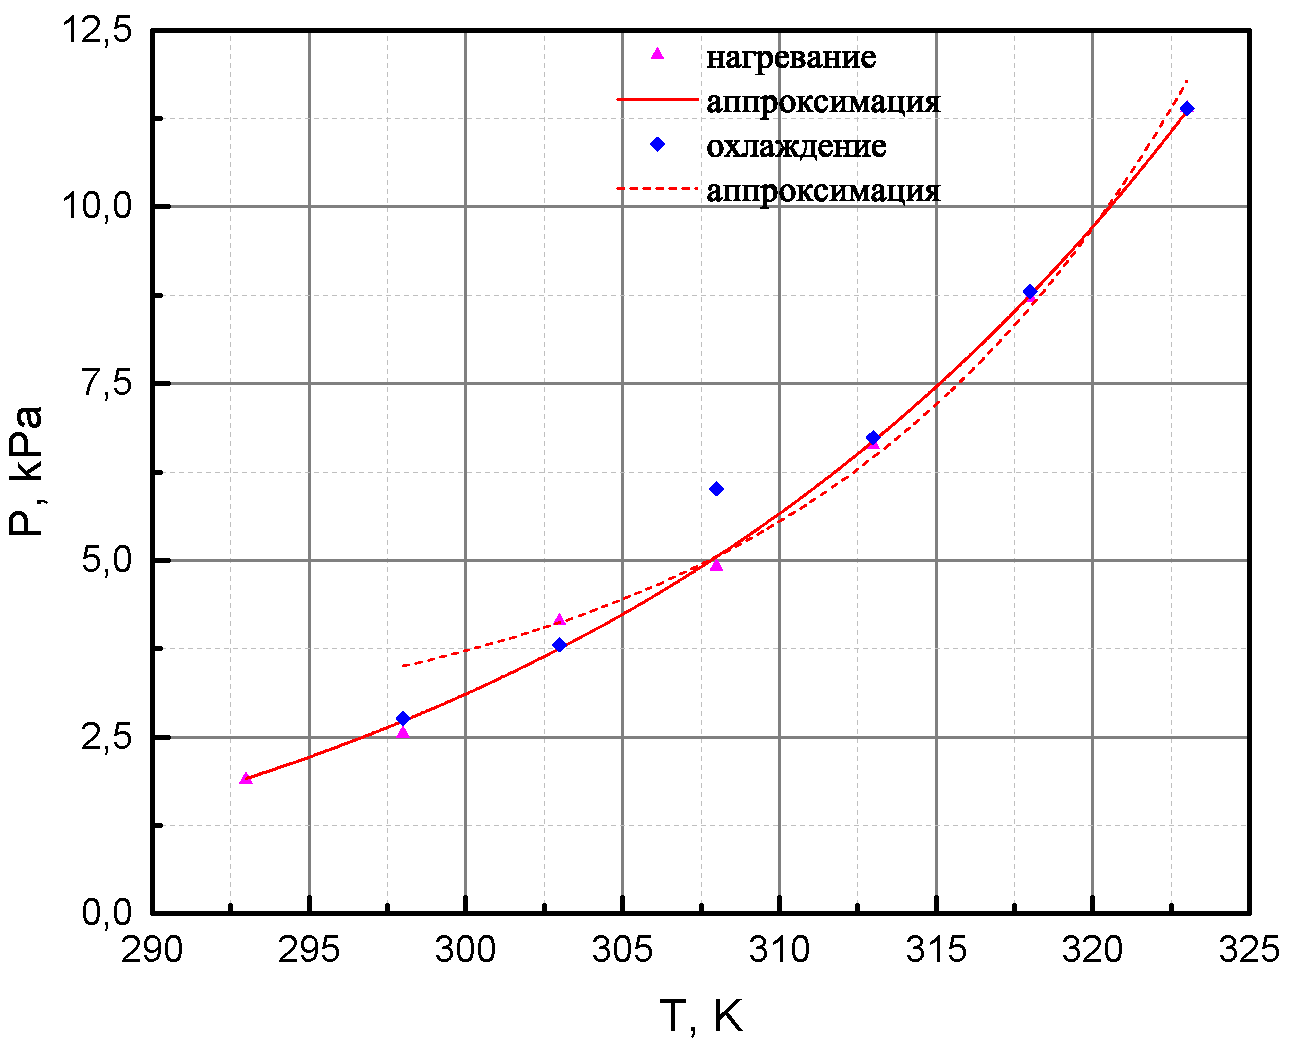
\includegraphics[scale=0.5]{Graph_1.pdf}}
	\caption{$R = R(T)$.}
	\label{ris:Graph_1}
\end{figure}
	
		
\newpage
	Для анализа полученных кривых рассмотрим наши экспериментальные точки в координатах $(1/T, \ln P)$ (рис.~\ref{ris:Graph_2}). Линейную аппроксимацию произведем методом наименьших квадратов без учета погрешности измеряемых величин в силу их малости.


\begin{figure}[H]
	\center{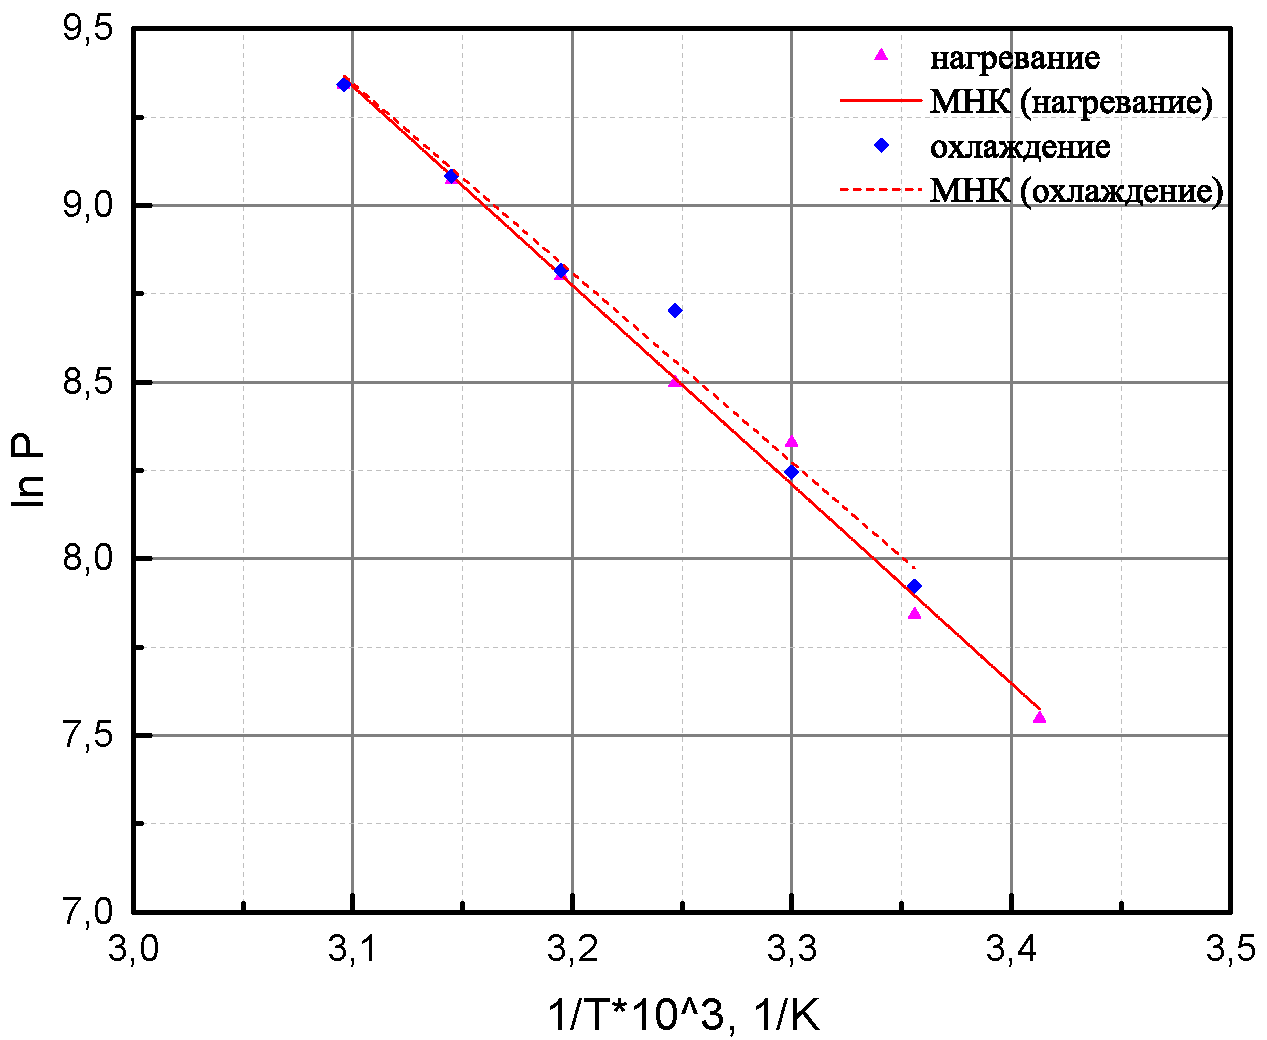
\includegraphics[scale=0.5]{Graph_2.pdf}}
	\caption{Зависимость $\ln P$ от $1/T$.}
	\label{ris:Graph_2}
\end{figure}


\floatsetup[table]{capposition=top}	
\begin{table}[H]
\caption{Результаты анализа прямых, представленных на рис.~\ref{ris:Graph_2}.}
\label{table:results_2}
\begin{tabular}{|c|c|c|c|c|}
\hline
$d\ln P / dT^{-1}$ & $\sigma_{d\ln P / dT^{-1}}$ & $L$, кДж/моль & $\sigma_L$, кДж/моль & $\varepsilon_L$, \% \\ \hline
-5,6               & 0,2                         & 47,0          & 1,7                  & 3,6                 \\ \hline
-5,4               & 0,4                         & 45,0          & 3,3                  & 7,3                 \\ \hline
\end{tabular}
\end{table}	

\section{Обсуждение результатов}
	С точки зрения равновесной термодинамики, тепловой эффект реакции, протекающей при постоянном давлении, равен изменению энтальпии системы: $Q_P = \Delta H$. Для расчета теплового эффекта при конкретной температуре можно применить уравнение Кирхгофа в интегральной форме:
\begin{equation}
	\Delta H_T^0 = \Delta H_{298}^0 + \int\limits_{298}^T \Delta C_P\,dT.
\end{equation}
	Откуда изменение энтальпии (теплота испарения) при фазовом переходе воды из жидкого агрегатного состояния в газовое:
\begin{equation}
	\label{entalpia}
	\Delta_f H_T^0 = \Delta_f H_{298}^0 - \Delta C_P (T-298),
\end{equation}
где $\Delta C_P = C_P^{\text{(г)}} - C_P^{\text{(ж)}}$, причём $C_P^{\text{(г)}} = C_P^{\text{(г)}} (T) = a + bT + c^\prime T^{-2}$. Приведем справочную таблицу~\ref{table:spravka}.

\floatsetup[table]{capposition=top}	
\begin{table}[H]
\caption{Термодинамические величины для воды.}
\label{table:spravka}
\begin{tabular}{|c|c|c|c|c|c|c|}
\hline
\multirow{3}{*}{Вещество} & \multirow{3}{*}{\begin{tabular}[c]{@{}c@{}}$\Delta_f H_{298}^0$,\\ кДж/моль\end{tabular}} & \multicolumn{4}{c|}{Теплоёмкость, Дж/моль$\cdot$К}                                       & \multirow{3}{*}{\begin{tabular}[c]{@{}c@{}}Температурный\\  интервал, К\end{tabular}} \\ \cline{3-6}
                          &                                                                                           & \multicolumn{3}{c|}{Коэффициенты ур-я $C_P^0 = f(T)$} & \multirow{2}{*}{$C_{P,\,298}^0$} &                                                                                       \\ \cline{3-5}
                          &                                                                                           & $a$   & $b \cdot 10^3$   & $c^\prime \cdot 10^{-5}$   &                                  &                                                                                       \\ \hline
$H_2O^{(\text{г})}$       & -241,84                                                                                   & 30    & 10,71            & 0,33                       & 33,56                            & 298-2500                                                                              \\ \hline
$H_2O^{(\text{ж})}$       & -285,84                                                                                   & -     & -                & -                          & 75,31                            & 298                                                                                   \\ \hline
\end{tabular}
\end{table}
	Используя формулу~(\ref{entalpia}) и таблицу~\ref{table:spravka} получим зависимость теплоты испарения воды от температуры:
\begin{equation}
	\label{tocn_formula}
	L\,[\text{Дж/моль}] = 44000 - (45,31 - 10,71 \cdot 10^{-3} \cdot T/[T] - 0,33 \cdot 10^5 \cdot [T^2]/T^2)(T/[T]-298)
\end{equation}

	Вычислим теплоту испарения по формуле~(\ref{tocn_formula}) при $T = 318$ К: $L = 43,173$ кДж/моль. Но экспериментально полученный нами результат $L = (47,0 \pm 1,7)$ кДж/моль был рассчитан в предположении, что в диапазоне температур от 293 К до 323 К теплоту испарения можно считать постоянной. Расхождение численных расчетов лишь подтверждает сильную зависимость $L = L(T)$, то есть формулу~(\ref{tocn_formula}). В этом случае наш результат завышен на 9\%, можно убедиться, что если мы рассчитаем $L$ при $T = 318$ К по приближенной формуле, но более точной в том смысле, что приращение температуры мало, то получим менее завышенный результат: $L \approx \frac{RT^2}{P} \frac{\Delta P}{\Delta T} = 45,1$ кДж/моль (завышен на 4,5\%). Стоит отметить, что при охлаждении мы получили большую погрешность измерений. Увеличение погрешности может быть связано с уменьшением количества экспериментальных точек и тепловой инерционностью ртути.
	
	Для повышения точности результатов, во-первых, необходимо уменьшить диапазон температур, в пределах которого рассчитываем теплоту испарения для опредленной температуры, во-вторых, можно учесть влияния насыщенного пара ртути, увеличения конденсата воды, изменения плотности ртути при нагревании.
	
\section{Выводы}
\begin{enumerate}
\item
	Нагревательный метод опредления теплоты испарения оказывается более эффективным.
\item
	Сравним экспериментальное значение теплоты испарения с теоретическим, убедились в ложности утверждения, что теплоту парообразования можно считать постоянной в диапазоне температур от 293 К до 323 К. 
\item
	Теплота испарения сильно зависит от температуры.

\end{enumerate}


\end{document}
